% coding:utf-8
\section{Fourierreihen}

\subsection{gerade oder ungerade Funktionen}

\subsubsection{Gerade Funktion: }
\[ \boxed{f(-x) = f(x)} \]
Die Funktion ist an der y-Achse gespiegelt. 
\subsubsection{Ungerade Funktion: }
\[ \boxed{f(-x) = -f(x)} \]
Die Funktion wird am Koordinatenursprung um 180° gedreht. 
\subsubsection{Achtung: }
Wichtig ist dabei, dass die Funktion erst nach der Erweiterung auf ganz $\mathbf{R}$ darauf geprüft wird, ob sie gerade oder ungerade ist. \\
So ist $\sin(x)$ eine ungerade Funktion. Wird jedoch nur die Periode $[0, \pi]$ betrachtet, so ist dies eine gerade Funktion. 

\begin{figure}[h!]
\centering
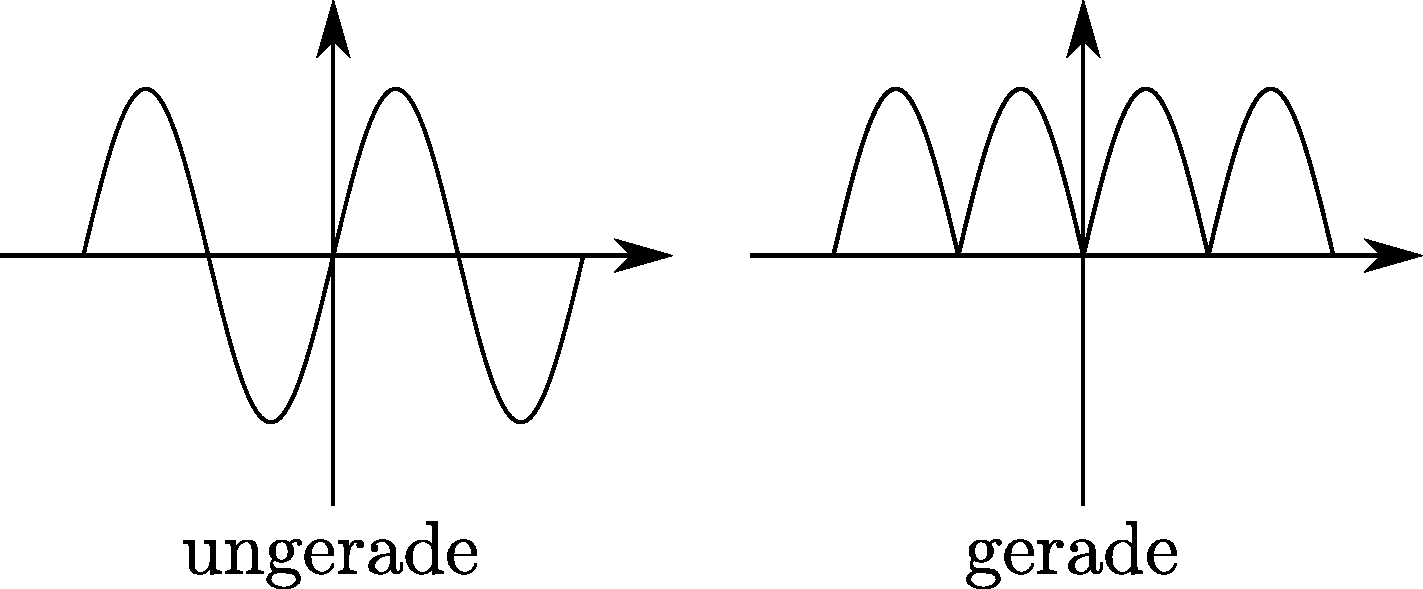
\includegraphics[width=0.7\textwidth]{geradeungerade.pdf}
\end{figure}

\subsection{n-te Partialsumme einer Fourierreihe für die Periode $2\pi$}
Die folgende Fourierreihe besitzt eine Periode von 2 $\pi$. 
\[ \boxed{f_n(x) = \frac{a_0}{2} + \sum_{K=1}^n \left(a_k \cdot \cos(kx) + b_k \cdot \sin(Kx)\right)} \]

\subsection{Koeffizienten für die Periode $2\pi$}
\[ \boxed{a_n = \frac{1}{\pi} \int_0^{2 \pi} f(x) \cos(nx) dx} \]
\[ \boxed{b_n = \frac{1}{\pi} \int_0^{2 \pi} f(x) \sin(nx) dx} \]
\[ \boxed{a_0 = \frac{1}{\pi} \int_0^{2 \pi} f(x) dx
} \]
Ist $f$ eine ungerade Funktion d.h. $f(-x) = -f(x)$, so gilt, da der $\cos(x)$ eine gerade Funktion ist: 
\[ a_k \equiv 0 \quad \forall K\]
\[ a_0 \equiv 0 \]
Ist $f$ eine gerade Funktion: 
\[ b_k \equiv 0 \quad \forall K \]

\subsection{n-te Partialsumme für die Periode T}
\[ \boxed{f_n(x) = \frac{a_0}{2} + \sum_{K=1}^n \left(a_k \cdot \cos \left(\frac{2 \pi}{T} K x\right) + b_k \cdot \sin\left(\frac{2 \pi}{T} K x\right)\right)} \]

\subsection{Koeffizienten für die Periode T}
\[ \boxed{a_n = \frac{2}{T} \int_T f(x) \cos(\frac{2 \pi}{T} K x) dx} \]
\[ \boxed{b_n = \frac{2}{T} \int_T f(x) \sin(\frac{2 \pi}{T} K x) dx} \]
\[ \boxed{a_0 = \frac{2}{T} \int_T f(x) dx
} \]

\subsection{Kochrezept zu Fourierreihen}
\begin{enumerate}
  \item Funktion auf ganz $\mathbf{R}$ fortsetzen
  \item Bestimmung, ob gerade oder ungerade Funktion\\
  f ungerade: $a_0, a_k = 0$\\
  f gerade: $b_k = 0$
  \item Periode bestimmen
  \item $a_0, a_k$ und $b_k$ berechnen
  \item n-te trigonometrische Summe zu f hinschreiben
\end{enumerate}

% \ifti
% \subsection{Fourierreihe mit dem TI-89 berechnen}
% \begin{verbatim}
% \integrate{}
% \end{verbatim}
% \fi
% \ifnspire
% \subsection{Fourierreihe mit dem TI-Nspire berechnen}

% \fi
